\chapter{Motorisation}
\label{chapter1}

Le projet repose sur un projet de telescope manuel, qui devait être placé à la main pour viser les étoiles.
Nous allons voire ici les choix et mises en oeuvre réalisé pour automatiser notre télescope.

\section{Placement des moteurs}

Le télescope est composé de deux axes à automatiser: la rotation et l'inclinaison. 

\begin{figure}[H]
    \centering
	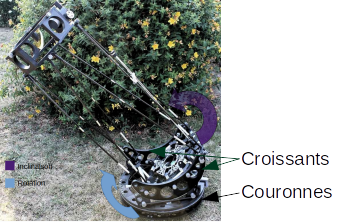
\includegraphics[width=0.49\linewidth]{\figures/Axe_rotation_telescope.png}
    \decoRule
    \caption[
    Illustration des axes telescope]{
    Illustration des axes telescope}
    \label{fig:Illustration des axes telescope}
    \end{figure}

Pour mouvoir le telescope en rotation, nous avons choisi de placer un moteur sur la couronne fixe à la base du telescope. Qui ce dernier ferai tourner la couronne du dessus qui sera équipée d'une courroie sur ça face intérieure. 

\begin{figure}[H]
    \centering
	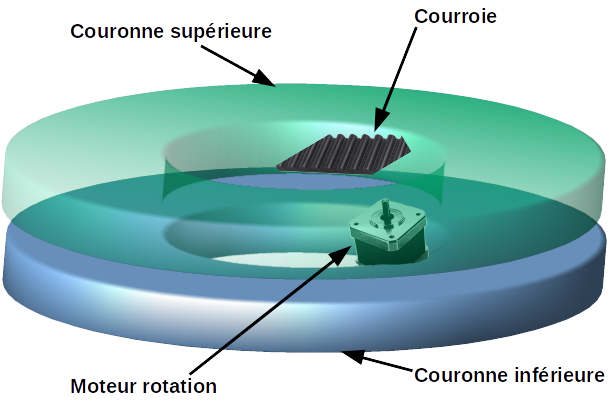
\includegraphics[width=0.49\linewidth]{\figures/illustration_rotation.png}
    \decoRule
    \caption[
    Illustration placement moteur rotation]{
    Illustration placement moteur rotation}
    \label{fig:Illustration placement moteur rotation}
    \end{figure}
    
Avant de choisir cette soluction nous avions réfléchi sur plusieurs autres. Nous avions envisagé de placer une courroie sur la face intérieur du croissant. La forme non-circulaire de l'interieur du croissant empêche de placer un axe FIXE pour entrainer une courroie car la forme du croissant va rapprocher la courroie de l'arbre du moteur durant ça progression.
Une autre solution visée à placer le moteur au centre de la courroie, cependant nous avons conclus que la surface sur laquelle va s'appliquer la force du moteur est plus petite que dans la solution que nous avons retenue.
\newline
\newline
Pour agir sur l'inclinaison, nous relions les deux barres qui maintiennent les croissants avec une courroie. Elle sera tendu grâce à l'arbre du moteur et un pignion. Le tout sera placé entre des deux croissants, sous le miroire principale.

\begin{figure}[H]
    \centering
	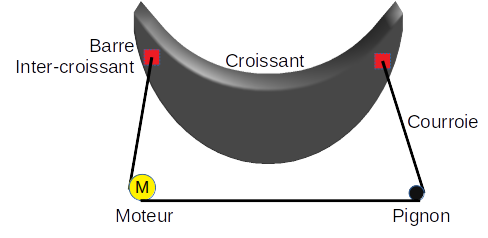
\includegraphics[width=0.49\linewidth]{\figures/Placement_moteur_inclinaison.png}
    \decoRule
    \caption[
    Illustration placement moteur inclinaison]{
    Illustration placement moteur inclinaison}
    \label{fig:Illustration placement moteur inclinaison}
    \end{figure}
    
Il nous reste ensuite une dernière chose à automatiser, le zoom. Le zoom sera placé entre le miroire secondaire et la caméra. Il sera entouré par une courroie qui fera le lien entre le zoom et une autre courroie entrainé par le moteur zoom.

\begin{figure}[H]
    \centering
	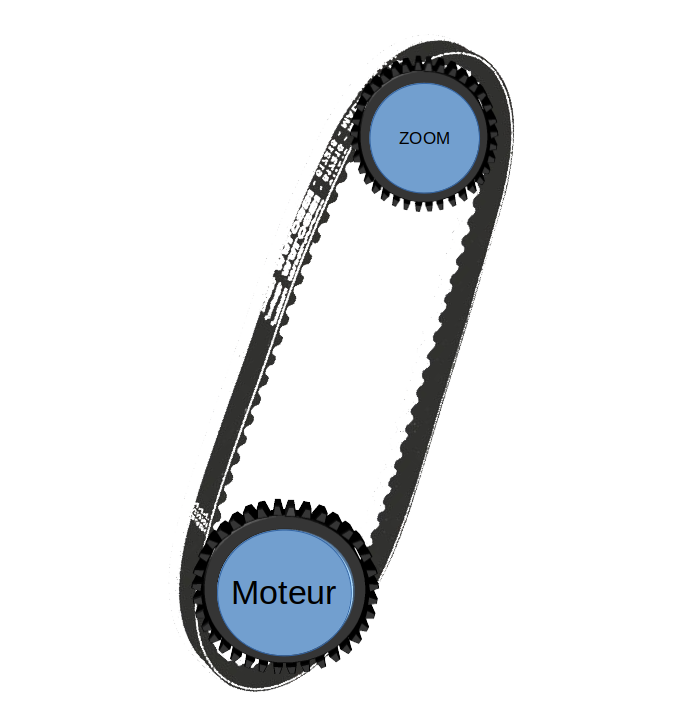
\includegraphics[width=0.49\linewidth]{\figures/Illistration_moteur_zoom.png}
    \decoRule
    \caption[
    Illistration moteur zoom]{
    Illistration moteur zoom}
    \label{fig:Illistration moteur zoom}
    \end{figure}

\section{Choix des moteurs}

D'après la quantité de matière au bout du télescope,et les matériels qui seront installés au bout (miroire, zoom, caméra, moteur pour le zoom, fixation) nous avons estimé que le moteur doit pouvoir soulever au minimum 4 kilogrammes.
Nous avons donc choisi le moteur de référence: 17HM15-0904S pour ça puissance et son coût. De plus nous disposions d'un tel moteur, avec lequel nous avons pu réaliser des testes pour nous assurer qu'il réponde bien à notre cahier des charges.
Le moteur du zoom a besoin de moins d'énergie pour agir sur le zoom, nous avons donc choisi un moteur moins puissant, celui retenu est le S20TH30-0604A.

\begin{figure}[H]
    \centering
	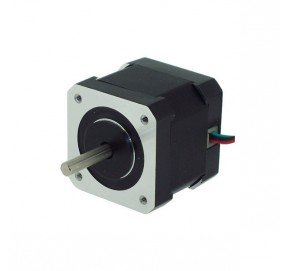
\includegraphics[width=0.49\linewidth]{\figures/moteur.jpg}
    \decoRule
    \caption[
    Photo du moteur]{
    Photo du moteur}
    \label{fig:Photo du moteur}
    \end{figure}
    
\section{Contrôle des moteurs}

Pour contrôler le moteur nous avons choisi le composant "A4988 Stepper Motor Driver Carrier". Il permet de contrôler la rotation du moteur, choisir entre le mode pas, demi-pas, quart de pas, huitième de pas et seizième de pas. Il y a également une pin activation et endormissement mais que nous n'utiliserons pas.

\begin{figure}[H]
    \centering
	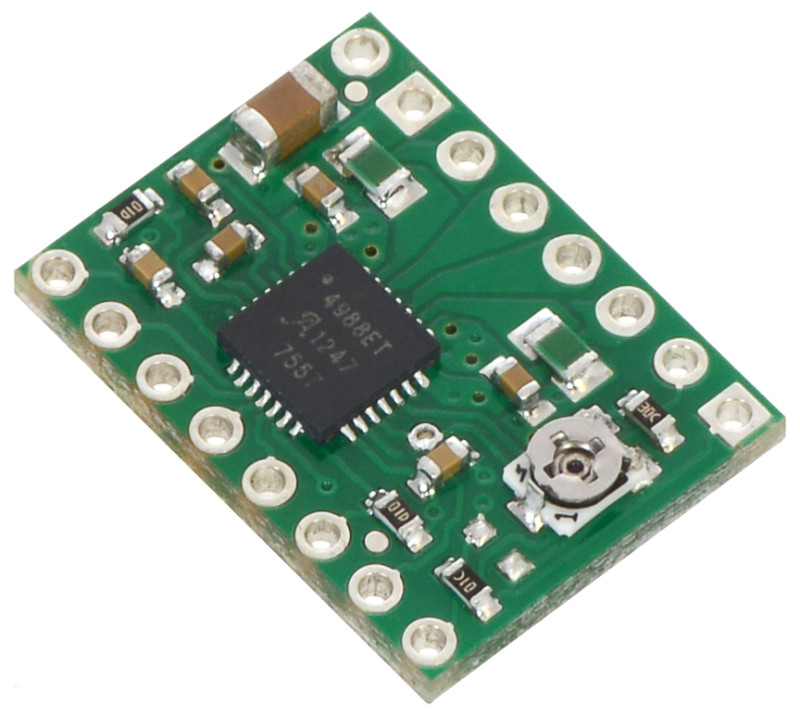
\includegraphics[width=0.49\linewidth]{\figures/controleur.jpg}
    \decoRule
    \caption[
    Photo du controleur]{
    Photo du controleur}
    \label{fig:Photo du controleur}
    \end{figure}


\section{Présentation du code}

Je développe un C un driver linux pour permettre le contrôle des moteurs, mais également de surveiller des interrupteurs, ces derniers serviront de capteur de fin de course. \newline
Le choix de réaliser un drive linux au lieu d'un logiciel est justifié parcequ'il permettra à un programme en couche supérieure d'utiliser ces fonctions pour mouvoir les moteurs.\newline
Pour contrôler les moteurs il faut générer une impultion, à chaque front montant le moteur réalise un pas s'il se trouve dans le mode pas à pas, sinon un demi-pas etc. Il faut également choisir le sens de rotation du moteur. \newline \newline
Fonctionnement: \newline
Lors de l'initialisation du drive l'interruptions de chacun des interrupteurs se mette en service, dès lors si l'un des interrupteurs placés en fin de course de la rotation s'active alors le moteur de rotation est immédiatement arrêté. Il en est de même pour l'inclinaison. Cette partie est autonome, et ne doit pas être utilisé par des logiciles tiers, c'est une sécurité matérielle. A l'inverse du contrôle des moteurs. Car chaque moteur dispose d'un fonction qui sera appelé par un logiciel tiers pour lancer un moteur sur un certain nombre de pas et dans une certaine direction.
\newline \newline
Avancement:\newline
Le contrôle des moteurs rotation et inclinaison sont réalisés. Les interruptions des interrupteurs de rotations sont également réalisées.
\newline \newline
Travail à venir:\newline
Réalisation du code permettant de contrôler le moteur zoom, et réalisation des interruptions des capteurs fin de course pour l'inclinaison et le zoom. \newline
Contrôle des modes des moteurs (mode de pas) en fonction de la distance à parcourir. Quand le moteur s'approche de la fin on réduit la taille des pas pour augmenter la précision, afin d'arriver exactement là où il faut.\newline

\section{En soutien}

J'ai participer en soutien dans la partie optique.\newline
Pour cela j'ai démarché plusieures entreprises dans le domaine de l'optique tel que STEMMER IMAGING S.A.S dont Alexis Bouras Ingénieur Technico-Commercial / Région Sud-Ouest, ce dernier m'a explique en fonction de nos contraites et materiels ce qu'il nous faut comme technologie réellement. J'ai également pris contact avec un amis travaillant dans le domaine. \newline
J'en ai conclus qu'il nous faut un zoom variable et qu'une focale variable nous est inutile.


